%% Eccentric MBH mergers and a search for semi-relativistic hypervelocity stars
%% AASTeX v7.0.1 -- ApJL format.
%% Compile: pdflatex, bibtex, pdflatex x2.
%% Requires f1.pdf, f2.pdf, bibliography.bib, and aasjournalv7.bst.
\documentclass[twocolumn]{aastex701}

\newcommand{\vinf}{v_{\infty}}
\newcommand{\kms}{\,{\rm km\,s^{-1}}}
\newcommand{\Msun}{\,M_{\odot}}
\newcommand{\rg}{r_{{\rm g},1}}
\defcitealias{gl15}{GL15}
\defcitealias{rotac25}{ROTAC}
\shorttitle{Searching for Semi-relativistic Hypervelocity Stars}
\shortauthors{Guillochon \& Loeb}

\begin{document}

\title{Searching for Semi-relativistic Hypervelocity Stars with
\textit{Euclid} and \textit{Roman}}

\correspondingauthor{James Guillochon}

\author[0000-0002-9809-8215]{James Guillochon}
\affiliation{Gentleman Astrophysicist}
\email[show]{guillochon@gmail.com}

\author[0000-0003-4330-287X]{Abraham Loeb}
\affiliation{Astronomy Department, Harvard University, 60 Garden Street,
Cambridge, MA 02138, USA}
\email{aloeb@cfa.harvard.edu}

\begin{abstract}
In 2015 we predicted that mergers of massive black hole (MBH) binaries launch
stars into intergalactic space at $10^{4}$--$10^{5}\kms$
($\approx0.03$--$0.3c$), and that hundreds of these semi-relativistic
hypervelocity stars (SHS) would be detectable in infrared surveys.
No searches so far have revealed any such stars. We revisit the prediction
in light of two developments. First, $e\gtrsim0.5$ during hardening is now a
result: circumbinary disks settle
at $e_{\rm eq}\simeq0.45$--$0.5$ rather than circularizing, while retrograde
disks pump toward $e\sim1$. Pulsar timing arrays prefer a low-frequency
turnover from environmental coupling, of which stellar slingshots are one
leading interpretation. Second, the ejection speed depends almost entirely
on the periapse, $\vinf\propto(r_{p}/\rg)^{-1/2}$, independent of primary
mass except as limited by tides. At fixed semimajor axis, $e=0.5$ raises
$\vinf$ by $\sqrt{2}$; $e=0.9$ by $\sqrt{10}$. \textit{Euclid} and \textit{Roman}
both provide near-infrared imaging that yields photometric
candidates, and slitless grism spectroscopy that verifies the bright tail.
Photometry does not identify them. \textit{Euclid}'s Wide Survey yields
$\approx140$ photometric detections at $H\simeq24$ over $14{,}000$ deg$^{2}$;
\textit{Roman}'s High-Latitude Wide-Area Survey goes deeper, yielding
$10^{2}$--$10^{3}$. Continuum detections in the two grisms are
$\approx0.3$ at \textit{Euclid} $H=19.5$ and $\approx0.4$ at \textit{Roman}
$m_{\rm AB}\approx21$; a velocity from bandheads is typically $0.5$--$1$~mag
brighter, so the completed surveys yield of order $0.1$--$0.5$. A $5\sigma$
Rubin proper motion in $r$ with a \textit{Roman} photometric distance reaches
$\approx0.4$ objects on the HLWAS footprint. A blueshifted photospheric
spectrum would verify an SHS; a proper motion large for that distance, with
no parallax, would do so jointly.
\end{abstract}

\keywords{Hypervelocity stars (776) --- Supermassive black holes (1663) ---
Galaxy mergers (608) --- Intergalactic medium (813) --- Sky surveys (1464)}

%%%%%%%%%%%%%%%%%%%%%%%%%%%%%%%%%%%%%%%%%%%%%%%%%%%%%%%%%%%%%%%%%%%%%%%%%
\section{Introduction}
\label{sec:intro}

Stars ejected by the Hills \citep{hills88} mechanism from the Galactic center
reach speeds of a few hundred to $\sim\!1700\kms$
\citep{brown05,brown15,koposov20}. In \citet[hereafter
\citetalias{gl15}]{gl15} and \citet{gl14} we pointed out that replacing the single massive
black hole with a \emph{merging} MBH binary
removes the limitation that sets this ceiling. A star bound to the secondary is
stripped when the secondary's Hill sphere shrinks below its orbital separation;
if the binary is eccentric, the last stars to be released are those most tightly
bound, and they leave with asymptotic speeds $\vinf$ that can exceed
$10^{4}\kms$ ($\approx0.03c$) and in principle approach $c/2$. Because no
other astrophysical channel produces unbound stars above
$\approx 2.4\times10^{4}\kms$ \citep{sari10,ginsburg12}, the detection of even
one such object would be a direct diagnostic of an eccentric MBH merger.

We estimated that $\sim\!10^{6}$ objects with $\vinf>10^{4}\kms$ lie within the
distance to the Virgo cluster, that roughly one SHS per 100 deg$^{2}$ would be
detectable in a survey reaching $K=24$, and that a next-generation wide-field
infrared mission would yield tens to hundreds of detections. No searches so
far have revealed any such stars.

\textit{Euclid} is mapping $\sim\!14{,}000$ deg$^{2}$ over a six-year survey
with slitless near-infrared spectroscopy \citep{euclid25}; the
\textit{Nancy Grace Roman Space Telescope} launches this month; the Vera C.\
Rubin Observatory began its survey two months earlier and has no astrometric
baseline; \textit{Gaia} DR4 has not yet been released.

The purpose of this paper is to make the case that the search should now be
performed, and to specify how candidates can be \emph{verified}. In
\S\ref{sec:speed} we restate the ejection kinematics of
\citetalias{gl15} in abbreviated form, reducing them to a single scaling in the
binary periapse and quantifying the effect of eccentricity on $\vinf$ and on counts. In \S\ref{sec:ecc} we
review the evidence, accumulated since 2015, that MBH binaries are eccentric
during the phase that matters. In \S\ref{sec:null} we explain why the Galactic
hypervelocity star null results do not constrain this population. In
\S\ref{sec:search} we give a concrete search: photometric detections in
\textit{Euclid} and \textit{Roman} imaging, verified by a grism radial
velocity, a Rubin or \textit{Roman} proper motion, or both.

%%%%%%%%%%%%%%%%%%%%%%%%%%%%%%%%%%%%%%%%%%%%%%%%%%%%%%%%%%%%%%%%%%%%%%%%%
\section{Ejection Speed is Set by the Periapse}
\label{sec:speed}

We collect the ejection kinematics of \citetalias{gl15} into a single
scaling with binary periapse, without repeating the scattering experiments.
Let the primary and secondary MBHs have masses $M_{1}$ and $M_{2}$, with
$q_{12}\equiv M_{1}/M_{2}>1$, and let the binary have semimajor axis $a$ and
eccentricity $e_{12}$, so that its periapse separation is
$r_{p}=a(1-e_{12})$. Stars bound to the secondary are removed when their
apoapse exceeds the secondary's Hill radius evaluated at binary periapse
\citepalias{gl15},
\begin{equation}
r_{H,e} = r_{p}\left(\frac{M_{2}}{3M_{1}}\right)^{1/3}.
\label{eq:hill}
\end{equation}
A star released from $a_{23}\simeq r_{H,e}$ has orbital speed
$v_{23}=(GM_{2}/a_{23})^{1/2}$ about the secondary and is ejected with
$\vinf \simeq 1.3\,q_{12}^{1/6}v_{23}$, where the numerical factor accounts for
the motion of the secondary at the moment of escape \citep{sari10}. Combining
these,
\begin{equation}
\vinf \simeq 1.3\times3^{1/6}\,q_{12}^{-1/6}\,
c\left(\frac{r_{p}}{\rg}\right)^{-1/2},
\label{eq:vinf}
\end{equation}
where $\rg\equiv GM_{1}/c^{2}$. Equation~(\ref{eq:vinf}) matches the mean
$\vinf/\langle v_{23}\rangle$ of the \citetalias{gl15} experiments, with large
scatter from orientation and phase. Numerically,
\begin{equation}
\vinf \simeq 0.19\,c
\left(\frac{r_{p}}{30\,\rg}\right)^{-1/2}
\left(\frac{q_{12}}{10}\right)^{-1/6}.
\label{eq:vinfnum}
\end{equation}

Equation~(\ref{eq:vinfnum}) has three immediate consequences. First, when the periapse is expressed in
gravitational radii of the primary, $\vinf$ is \emph{kinematically} independent
of $M_{1}$: the same periapse in units of $\rg$ yields the same ejection speed
for a $10^{7}\Msun$ and a $10^{9}\Msun$ primary. The \emph{accessible} range of
$r_{p}/\rg$ is not. For a solar-type star the tidal radius is
$r_{t}/\rg \approx 0.47\,(M_{1}/10^{9}\Msun)^{-2/3}$. The star's closest
approach to the primary is $r_{p}-a_{23}\approx0.68\,r_{p}$ at $q_{12}=10$, so
the innermost bound circular orbit (IBCO; $4\rg$ for Schwarzschild) lies
outside $r_{t}$ at that closest approach only for
$M_{1}\gtrsim7\times10^{7}\Msun$. Below that, the star is disrupted before it
can reach the periapse of the fastest ejections: at $M_{1}=10^{7}\Msun$,
$r_{t}\approx10\rg$ and the ceiling is $\vinf\approx0.27c$, not $c/2$. An
intact star at $r_{p}=280\rg$ around the $4\times10^{6}\Msun$ Galactic-center
primary \citep{gravity26} lies outside $r_{t}/\rg\approx19$ at
that mass, an empirical illustration of the same survival cut. Second, the
dependence on mass ratio is extremely weak, $q_{12}^{-1/6}$, so that a factor
of ten in $q_{12}$ changes $\vinf$ by only $32\%$. The near-coincidence of the
$c/2$ cap with the IBCO in Figure~\ref{fig:main}(a) is a property of
$q_{12}=10$; at $q_{12}=1$ the $c/2$ speed is reached at
$r_{p}\approx10\rg$, outside the IBCO, so the two ceilings are independent
and their ordering depends on $q_{12}$. At $r_{p}=30\rg$ the star already
orbits the secondary at $\approx0.1c$, so the upper-left corner of
Figure~\ref{fig:main}(a) is where the Newtonian treatment is least
trustworthy; the $c/2$ cap is the numerical and special-relativistic ceiling
of \citetalias{gl15}, not a Newtonian limit. A prograde orbit about a rapidly
spinning primary moves the IBCO inward toward $\sim\rg$ \citep{bardeen72},
which would raise the kinematic ceiling. Third, once
tidal survival is satisfied, $\vinf$ depends only on $r_{p}/\rg$. Reaching $\vinf>10^{4}\kms$ requires
$r_{p}\lesssim 10^{3}\rg$; reaching $\vinf>2.4\times10^{4}\kms$, above which no
other channel operates \citep{sari10,ginsburg12}, requires $r_{p}\lesssim 200\rg$.

Eccentricity enters only through $r_{p}=a(1-e_{12})$, but it enters
multiplicatively with the hardening. At a fixed stage of binary evolution,
\begin{equation}
\frac{\vinf(e_{12})}{\vinf(0)} = (1-e_{12})^{-1/2},
\label{eq:eboost}
\end{equation}
so $e_{12}=0.5$ raises the ejection speed by $\sqrt{2}$ and $e_{12}=0.9$ by
$\sqrt{10}$. Because the velocity distribution is steep, the effect on
detectable counts is larger than this suggests. For the differential
distribution $P(\vinf)\propto \vinf^{-2.5}$ of the MBH-scattering channel
\citep{sesana07,sherwin08} that \citetalias{gl15} found to describe the
population at several thousand $\kms$, the cumulative
$N(>\vinf)\propto \vinf^{-1.5}$, so the number above any fixed threshold
scales as
\begin{equation}
\frac{N(>\vinf;e_{12})}{N(>\vinf;0)}=(1-e_{12})^{-0.75},
\label{eq:nboost}
\end{equation}
a factor of $\approx1.7$ at $e_{12}=0.5$ and $\approx6$ at $e_{12}=0.9$.
This is a property of $P(\vinf)$, not a multiplier to apply on top of the
\citetalias{gl15} density, which already assumed $e_{12}\gtrsim0.5$.
\citetalias{gl15} found the slope to steepen at
higher velocities, which would only increase these factors.

Figure~\ref{fig:main}(a) shows $\vinf$ as a function of $e_{12}$ for three
hardening stages, for $M_{1}=10^{9}\Msun$ and $q_{12}=10$. Curves are truncated
where $r_{p}$ falls inside the innermost bound circular orbit
\citep{bardeen72} and capped at the $c/2$ speed limit identified in
\citetalias{gl15}. The figure shows that a binary
that has hardened to milliparsec separations reaches the
merger-only velocity regime across the range of eccentricities now predicted
at hardening.

\begin{figure*}[t]
\centering
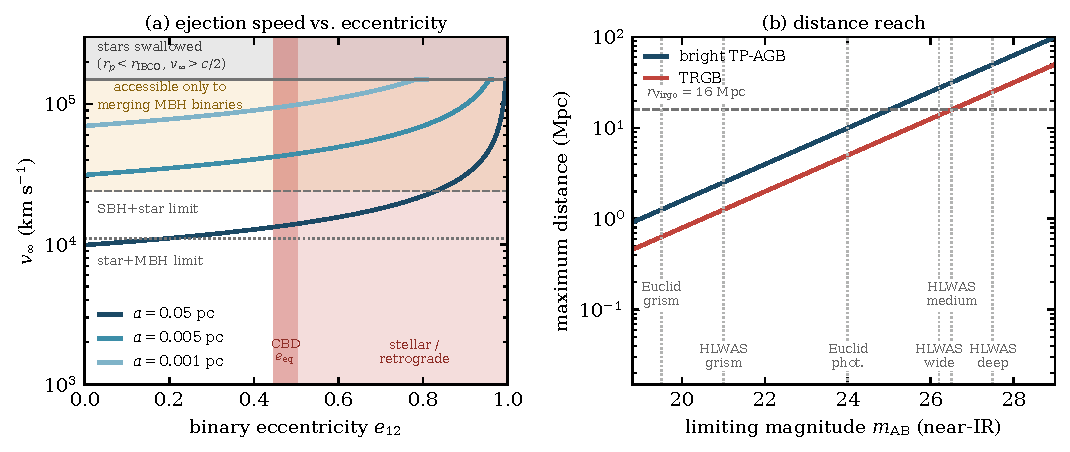
\includegraphics[width=\textwidth]{f1.pdf}
\caption{(a) Asymptotic ejection speed as a function of binary eccentricity for
three hardening stages ($M_{1}=10^{9}\Msun$, $q_{12}=10$), from
Equation~(\ref{eq:vinf}). Curves terminate where the periapse reaches the
innermost bound circular orbit \citep{bardeen72} and are capped at $c/2$.
At $q_{12}=10$ those two limits nearly coincide; they are independent
constraints whose ordering depends on mass ratio, and intact survival at
the IBCO periapse requires $M_{1}\gtrsim7\times10^{7}\Msun$ (see text).
The dotted and dashed lines mark the Hills-mechanism ceilings derived in
\citetalias{gl15} from the encounter kinematics of \citet{sari10}:
$1.1\times10^{4}\kms$ for a stellar binary and a single MBH
\citep[consistent with][]{ginsburg12}, and $2.4\times10^{4}\kms$ for a
stellar-mass black hole--star binary. The shaded region above is accessible
only to merging MBH binaries. The vertical band marks the
range of eccentricities now predicted during hardening: the circumbinary-disk
attractor $e_{\rm eq}\simeq0.45$--$0.5$ \citep{zrake21,siwek23,munoz19}, and the
higher values reached by stellar scattering and retrograde disks
\citep{iwasawa11,khan12,tiede24}. (b) Maximum distance at which a star of
given absolute magnitude is detected as a function of limiting near-infrared
magnitude, for two characteristic luminosities introduced here (the
tip of the red giant branch and bright TP-AGB stars) rather than the mixed
isochrone sample of \citetalias{gl15}. \textit{Euclid} $H$ and \textit{Roman}
F158 are treated as equivalent AB magnitudes. Vertical lines mark the
\textit{Euclid} and HLWAS grism continuum limits, \textit{Euclid}'s photometric
depth (the limit assumed in \citetalias{gl15}), and the HLWAS wide, medium, and
deep tiers. The dashed horizontal
line is the Virgo distance within which \citetalias{gl15} computed the
population, a computational boundary rather than a physical one.}
\label{fig:main}
\end{figure*}

%%%%%%%%%%%%%%%%%%%%%%%%%%%%%%%%%%%%%%%%%%%%%%%%%%%%%%%%%%%%%%%%%%%%%%%%%
\section{The Eccentric-Merger Premise Has Strengthened}
\label{sec:ecc}

In \citetalias{gl15}, the requirement that a significant fraction of MBH binaries
pass through a phase with $e_{12}\gtrsim0.5$ was the single largest source of
uncertainty in the predicted space density. At the time it rested on $N$-body
simulations of unequal-mass binaries embedded in stellar cusps
\citep{baumgardt06,iwasawa11,khan12} (the gas-poor channel), while the
gas-rich channel was less clear. Both now favor $e_{12}\gtrsim0.5$ during
hardening: stellar scattering still drives eccentricity growth
\citep{iwasawa11,khan12,sesana10}, and circumbinary disks evolve to
$e_{\rm eq}\simeq0.45$--$0.5$ (or higher if retrograde) rather than
circularizing \citep{zrake21,siwek23,munoz19,tiede24}.

\subsection{Gas does not circularize these binaries}

High-resolution hydrodynamic simulations of accreting binaries embedded in
circumbinary disks now consistently find that the orbit evolves toward a nonzero
\emph{equilibrium} eccentricity rather than toward zero.
\citet{zrake21} find $e_{\rm eq}\simeq0.45$ for equal-mass binaries, with
circularization only for orbits initialized at $e\lesssim0.08$.
\mbox{\citet{siwek23}}, in the largest parameter survey performed to date, find that
eccentricities evolve to steady-state values that increase with mass ratio and
saturate at $e_{\rm eq}\simeq0.5$, and that
binaries at their steady-state eccentricity with $q_{b}\gtrsim0.3$ continue to
evolve toward coalescence. \citet{munoz19} found eccentricity growth at
$e=0.1$ and damping at $e=0.5$--$0.6$, the sign change that implies an
attractor. \citet{tiede24} find that retrograde disks instead pump
eccentricity at every value they simulated ($0$--$0.8$), with $\dot{e}>0$
throughout and $e\rightarrow1$ in $\sim20$ Myr at Eddington accretion; such
high eccentricities would only raise $\vinf$ and, if the merger is plunging,
tighten the beaming that concentrates the local population toward a few
sources. See \citet{lai23} for a review.

Gas dynamics need not supply the extreme eccentricities of the fastest
ejections. It does mean that gas-rich MBH binaries are now expected to arrive
at the hardening phase eccentric, at values straddling the $e_{12}\gtrsim0.5$
threshold we required, and to remain so while they harden.

\subsection{Stellar dynamics drives eccentricity growth}

The stellar-dynamical channel identified before 2015 remains in place.
\citet{iwasawa11} showed that the secondary's eccentricity grows through the
preferential ejection of stars co-rotating with the binary, with the growth
halted only by the discreteness noise of the scattered stars; \citet{baumgardt06}
and \citet{khan12} found efficient, eccentric coalescence in merging galaxies.
Near-equal-mass binaries show only mild eccentricity growth
\citep{sesana10}, so the effect is strongest at intermediate mass ratios, which
is the regime that Equation~(\ref{eq:vinfnum}) shows to be most
favorable, since $\vinf\propto q_{12}^{-1/6}$ varies negligibly across it.

\subsection{Pulsar timing arrays see the ejection process itself}

The detection of a nanohertz stochastic gravitational-wave background
\citep{nanograv23} is consistent with a cosmological population of MBH binaries
\citep{agazie23b}. More directly relevant here, the measured spectrum shows a
preference for a turnover at the lowest observed frequencies, which is naturally
produced if the binaries are hardened by environmental coupling before
gravitational-wave emission takes over. \citet{chen26} attribute this turnover
specifically to the extraction of orbital energy by three-body slingshot
ejection of stars.

The process that the pulsar timing array data appear to require (three-body
stellar slingshots that extract orbital energy \citep{chen26,sesana10}) is the
same family of encounters that unbinds stars from merging MBH binaries. That is
indirect evidence that MBH binaries eject stars while they harden, not a
measurement of the SHS space density.

\subsection{A caveat on LISA-band eccentricities}

\citet{zrake21} predict that binaries entering the LISA band will retain only
$e\simeq10^{-3}$--$10^{-2}$. Gravitational-wave emission circularizes the
orbit efficiently \citep{peters64}, but it does so at separations far smaller
than those at which stars are stripped from the secondary's Hill sphere. The eccentricity relevant
to SHS production is that of the hardening phase at $\sim10^{-3}$--$10^{-1}$ pc
\citep{sesana10,tiede24},
not the residual eccentricity at merger. Low LISA-band eccentricities and high
hardening-phase eccentricities are entirely compatible, and both are predicted
by the same simulations.

%%%%%%%%%%%%%%%%%%%%%%%%%%%%%%%%%%%%%%%%%%%%%%%%%%%%%%%%%%%%%%%%%%%%%%%%%
\section{Galactic Null Results Do Not Apply}
\label{sec:null}

The strongest empirical statements about hypervelocity star production come from
\textit{Gaia}. \citet{marchetti22} searched the $\sim\!34$ million DR3 sources
with full six-dimensional phase-space information and found no candidate above
$700\kms$ with reliable six-dimensional kinematics, deriving an ejection rate
$\lesssim8\times10^{-5}\,{\rm yr^{-1}}$. \citet{verberne24} identified 600
candidates, obtained ground-based follow-up for 196, found no
new hypervelocity star, and constrained the ejection rate for stars above
$1\Msun$ to $<10^{-5}\,{\rm yr^{-1}}$ at $2\sigma$. \citet{evans23} used the
absence of candidates to exclude a companion to Sgr~A$^{*}$ more massive than
$2000\Msun$ within one milliparsec.

These do not bear on the SHS population, for three independent reasons:

\emph{Mechanism.} \citet{marchetti22} and \citet{verberne24} model Hills
ejection by a single MBH; \citet{evans23} consider a possible companion to
Sgr~A$^{*}$ but constrain it with the same Galactic hypervelocity-star sample.
The SHS channel requires an MBH \emph{merger}. The Milky Way is not undergoing
one; indeed \citet{evans23} conclude that Sgr~A$^{*}$ has had no companion more
massive than $500\Msun$ for at least 10 Myr, which is consistent with our
framework.

\emph{Volume.} The \textit{Gaia} 6D sample is confined to the Galaxy. The SHS
population is extragalactic, and in \citetalias{gl15} we speculated that if
ejections are beamed, the local density may originate from a couple of mergers,
illustrated with an event in M87. We predicted only $\sim\!10^{2}$ objects with
$\vinf>10^{4}\kms$ within 1 Mpc of the Milky Way, and those are predominantly
low-mass dwarfs requiring space-based depth.

\emph{Selection.} A star moving at $10^{4}\kms$ at a distance of 1 Mpc has a
proper motion of $2.1$ mas yr$^{-1}$; at 10 Mpc, $0.21$ mas yr$^{-1}$. Searches
that select on large proper motion combined with a measured radial velocity are
blind to such objects by construction.

%%%%%%%%%%%%%%%%%%%%%%%%%%%%%%%%%%%%%%%%%%%%%%%%%%%%%%%%%%%%%%%%%%%%%%%%%
\section{A Concrete Search with \textit{Euclid} and \textit{Roman}}
\label{sec:search}

Both missions provide wide-field
near-infrared imaging that yields photometric candidates, and slitless grism
spectroscopy that can verify the bright tail kinematically.

\textit{Euclid}'s Wide Survey maps $\sim\!14{,}000$ deg$^{2}$ to $H\simeq24$
with NISP slitless spectroscopy at $R\sim450$ over $1.21$--$1.89\,\mu$m
\citep{euclid25}, the Euclid-class limit assumed in \citetalias{gl15}.
That area is a six-year goal, not a current footprint: nominal survey
operations began in 2024 February, $5000$ deg$^{2}$ had been observed by
2026 March, and the Wide Survey completes around 2030. DR1 is scheduled for
2026 October.

The \textit{Roman} High-Latitude Wide-Area Survey (HLWAS) covers
$\approx4900$ deg$^{2}$ in three tiers \citepalias{rotac25}: a wide tier of
$\approx2500$ deg$^{2}$ reaching $m_{\rm AB}=26.2$ in F158; a medium tier of
$\approx2350$ deg$^{2}$ reaching $26.5$ mag (AB) in three filters,
with slitless grism spectroscopy over the same area; and a deep tier of
$19.2$ deg$^{2}$ (two fields of $\approx9.5$ deg$^{2}$) reaching about $1.1$ mag
deeper in F158 ($m_{\rm AB}\approx27.5$),
of which an ultra-deep component of $\approx5.5$ deg$^{2}$ reaches $28.2$.\footnote{STScI
\textit{Roman} User Documentation, ``High-Latitude Wide-Area Survey,''
\url{https://roman-docs.stsci.edu/roman-community-defined-surveys/high-latitude-wide-area-survey},
accessed 2026 August 29. Areas in the flight implementation are $2525$, $2356$,
and $19.2$ deg$^{2}$ for the wide, medium, and deep tiers; we round the first
two in the text. The design origin is \citetalias{rotac25}.}
The
wide-field instrument delivers a $0.28$ deg$^{2}$ field at $0\farcs11$
pixels \citep{akeson19}, and the grism spans $1.0$--$1.93\,\mu$m at resolving
power $R\approx475$--900 \citep{bray24}. The detection calculation below is
the same for both surveys; only the area and depth change. We treat
\textit{Euclid} $H$ and \textit{Roman} F158 as equivalent AB magnitudes.

\subsection{Photometric detections are candidates}

Rescaling our surface density of one SHS per $100$ deg$^{2}$ at the $H<24$
Euclid- or WFIRST-class limit of \citetalias{gl15} (AB in the survey papers
that set that cut; the introductory $K=24$ is the same infrared depth), and
splitting the detections as in \citetalias{gl15} (red-giant-branch stars
about half; the brighter giant branches the rest), gives a Euclidean surface
density that depends only on depth. We apply that density at \textit{Euclid}
$H$ and \textit{Roman} F158 with no $H-K$ offset. The circumbinary-disk
attractor confirms the $e_{12}\gtrsim0.5$ already assumed in
\citetalias{gl15} rather than raising the counts; retrograde $e_{12}=0.9$
can still sit a factor $\approx6$ above (Equation~(\ref{eq:nboost})). That
normalisation is inherited from \citetalias{gl15} and is unrevised;
merger-rate density, loss-cone supply, isochrone conversion, and the
high-velocity slope of $P(\vinf)$ each contribute uncertainties of order a
dex or more, larger than the eccentricity envelope itself.

SHS are not sourced only within $16$ Mpc.
A star at $0.03c$ travels $\approx130$ Mpc in a Hubble time, so the local
density is an integral over the merger history of a $\sim100$ Mpc sphere, and
there is no physical reason for it to fall off outside Virgo. We therefore take
Euclidean growth as the primary prediction, with the $r_{\rm Virgo}$
truncation of \citetalias{gl15} as a conservative floor. Applied to each
survey (Figure~\ref{fig:yield}): \textit{Euclid}'s $H\simeq24$ Wide Survey
recovers the original \citetalias{gl15} forecast, $\approx140$ photometric
detections over $14{,}000$ deg$^{2}$. The HLWAS wide tier, $2.2$ mag deeper,
contains $\approx530$; the medium tier, $0.3$ mag deeper still,
$\approx750$; the $19.2$ deg$^{2}$ deep tier, $1.1$ mag deeper in F158,
$\approx24$ rather than the $\approx4$ at which the truncated calculation
saturates, an order-of-magnitude increase, which is why we develop the
photometric selection there (\S\ref{sec:disc}).

These are faint red point sources, not identifications. As we noted in
\citetalias{gl15}, the color shift induced by bulk motion is only a few tenths
of a magnitude and is degenerate with normal giant-branch color evolution; the
sky is full of Galactic dwarfs and unresolved background galaxies. An SHS is
verified only when a velocity is measured: a grism radial velocity, a proper
motion from Rubin or \textit{Roman}, or both.

Figure~\ref{fig:yield} shows how the photometric counts depend on what is
assumed. A shared space density would place the TP-AGB curve a factor
$\approx8$ above the TRGB curve, the volume ratio implied by
$\Delta M=1.5$~mag in Figure~\ref{fig:main}(b). The two classes are not
equally abundant. In \citetalias{gl15}, red-giant-branch stars were about half
of the detections at $H=24$, with the shorter-lived, brighter giant branches
contributing the rest. Matching that mix at $m=24$ implies a TP-AGB space
density lower by $(d_{\rm TP-AGB}/d_{\rm TRGB})^{3}\approx8$, so the
Euclidean rises coincide: the extra volume and the lower density cancel.
They peel apart only if each tracer is capped at $r_{\rm Virgo}$ (TP-AGB at
$m_{\rm AB}\approx25$, TRGB at $\approx26.5$), which we treat as a floor
rather than the prediction. The shaded envelope is the eccentricity
systematic alone, spanning $e_{12}=0$ (a factor $1.7$ below the fiducial) to
$e_{12}=0.9$ (a factor $\approx6$ above, the retrograde-disk channel of
\citealt{tiede24}); it is not an error budget. A realistic photometric sample
is of order $10^{2}$--$10^{3}$. The kinematically verifiable subset is the
nearby, brighter tail of that distribution.

We bound the same volume with two characteristic luminosities rather than
the mixed isochrone sample of \citetalias{gl15}. In \citetalias{gl15} we
converted the kinematic population with stellar isochrones and a Kroupa IMF
at an $H<24$ (WFIRST- or Euclid-class) limit, without separating the tip of
the red giant branch from the TP-AGB. We convert that mix into space
densities so that the brighter class is not treated as equally numerous.
Taking $M_{\rm AB}\simeq-4.5$ for the TRGB
\citep{newman24} and $M_{\rm AB}\simeq-6$ for luminous TP-AGB stars
\citep{madore20}, \textit{Euclid} at $H=24$ reaches $5.0$ and $10$~Mpc;
HLWAS wide reaches $13.8$ and $27.5$~Mpc, and the deep tier $25$~Mpc for the
TRGB (Figure~\ref{fig:main}b). Both surveys detect evolved SHS throughout
and well beyond the $r_{\rm Virgo}=16$ Mpc volume within which
\citetalias{gl15} computed the population; as argued above, that volume is a
computational boundary rather than a physical one. Most of those detections
will not have a measured velocity.

The sky distribution need not be isotropic. In \citetalias{gl15} the counts
assumed an isotropic distribution, but we also noted that if mergers are
plunging, the local population may originate from only a couple of events, and
illustrated the case of a merger in M87 whose debris streams toward the Milky
Way rather than filling the sky uniformly. The two deep-tier fields, COSMOS and XMM-LSS, lie $39^{\circ}$ and
$151^{\circ}$ from M87; each sits inside one of the two medium-tier
footprints. For stars streaming
radially from $D=16$ Mpc with a density falling as $R^{-2}$, the two carry
weights of $1.9$ and $0.35$ relative to the all-sky mean. Because they lie on
opposite sides of the sky the summed yield moves by less than $15\%$. The photometric rates above are
therefore insensitive to whether the sources are isotropic or Virgo-dominated,
even though the field-to-field split is not.

\begin{figure}[t]
\centering
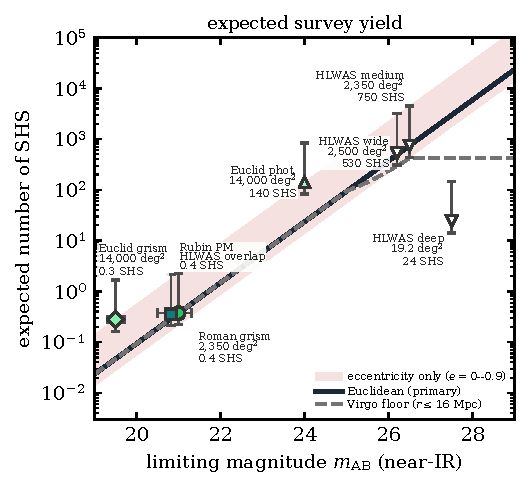
\includegraphics[width=\columnwidth]{f2.pdf}
\caption{Expected number of SHS as a function of survey depth.
The solid curve is Euclidean growth of the unboosted
\citetalias{gl15} density (one SHS per $100$ deg$^{2}$ at $H=24$), the
primary prediction; the dashed curve caps each tracer at $r_{\rm Virgo}$ and
is a conservative floor. Open symbols are photometric detections (\textit{Euclid} Wide and HLWAS
tiers); filled symbols are kinematic searches
(\textit{Euclid} and \textit{Roman} grism continuum limits; Rubin $5\sigma$
proper motions in $r$ on the HLWAS footprint). The Euclid grism bar is the
published $\pm0.2$ mag on $H=19.5$. Grism markers sit at the published
continuum depths; a velocity from bandheads is typically $0.5$--$1$~mag
brighter (see text). Vertical bars and the shaded band span the eccentricity
systematic only, from $e_{12}=0$ to $e_{12}=0.9$; they are not a full error
budget. Each survey is labeled with its name, area, and expected count.}
\label{fig:yield}
\end{figure}

\subsection{Radial velocities: the grisms}

Both surveys disperse every source on the detector. At $R\sim450$
(\textit{Euclid}/NISP) to $R\approx600$ (HLWAS), a bulk velocity of
$10^{4}\kms$ displaces spectral features by $\approx15$--$20$ resolution
elements, $5000\kms$ by $\approx7.5$--$10$, and $3000\kms$ by
$\approx4.5$--$6$. In slitless spectroscopy the wavelength zero-point is
set by the source's position along the dispersion direction, so
$\lambda_{0}$ requires astrometric registration to $\lesssim1$ NISP pixel
($\approx670\kms$ at $R\sim450$); that is why we lead with
$10^{4}\kms$, the velocity at which no competing channel operates. A
stellar photospheric spectrum, with the CO bandheads near $1.6\,\mu$m and
CN near $1.1\,\mu$m, is unmistakable against the smooth continuum of a
background galaxy, and a \emph{blueshifted} stellar spectrum has no
astrophysical contaminant at all. That is a radial-velocity verification,
obtained from the same exposures taken to measure galaxy H$\alpha$
redshifts.

The continuum limit is the binding constraint, and it is where the two
surveys trade area against depth. The published NISP $3.5\sigma$ continuum
is $H=19.5\pm0.2$ for compact galaxies \citep{euclid23grism}; NISP
undersamples the PSF ($0\farcs3$ pixels), so that limit is already close to
the point-source depth relevant for SHS. For HLWAS, the published one-hour
point-source continuum limits at $1.5\,\mu$m are $m_{\rm AB}=21.3$
($5\sigma$ per pixel) and $20.5$ ($10\sigma$ per pixel)
\citep{akeson19}.\footnote{NASA GSFC, ``Wide Field Instrument
Technical,'' \url{https://roman.gsfc.nasa.gov/science/WFI_technical.html},
and STScI \textit{Roman} User Documentation, ``WFI Quick Reference,''
\url{https://roman-docs.stsci.edu}, both give $m_{\rm AB}=21.3$ (5$\sigma$
per pixel) at $1.5\,\mu$m in 1~hr. \citet{akeson19} quote $20.5$ at
10$\sigma$ per pixel in the same time at $1.5\,\mu$m. Those tables assume
twice the minimum zodiacal background; typical HLWAS backgrounds are
$\sim30\%$ lower.}
The medium-tier grism stack is $4$ passes of $2\times190$~s dithers, or
$1520$~s on source. Scaling the $5\sigma$ per-pixel limit as
$f_{\rm lim}\propto t^{-1/2}b^{1/2}$ gives $m_{\rm AB}\approx20.8$ at the
table zodiacal level and $\approx20.9$ at typical HLWAS backgrounds,
confirming the $m_{\rm AB}\approx21$ threshold adopted below.

The same surface density then gives both continuum yields
(Figure~\ref{fig:yield}). At $H=19.5$, \textit{Euclid} reaches $0.63$~Mpc
(TRGB) and $1.3$~Mpc (TP-AGB); at $m_{\rm AB}\approx21$, HLWAS reaches
$1.3$ and $2.5$~Mpc. Counts scale as the cube of the distance, and
\textit{Euclid}'s sixfold area ($14{,}000$ vs.\ $2350$ deg$^{2}$) only just
cancels a $\approx1.3$ mag deficit, so the completed surveys yield
$\approx0.3$ and $\approx0.4$ continuum detections at those published
limits. A velocity from bandheads wants a signal-to-noise of a few per
resolution element, typically $0.5$--$1$~mag brighter, so the completed
surveys yield of order $0.1$--$0.5$ objects with a measured velocity, a few
at $e_{12}=0.9$. \textit{Euclid}'s total is not yet in hand: it accumulates at
$\approx2300$ deg$^{2}$ yr$^{-1}$, the $5000$ deg$^{2}$ observed by 2026
March contain $\approx0.1$ expected continuum objects, and the $O(1)$
spectroscopic yield arrives when the Wide Survey finishes around 2030. HLWAS is slightly deeper and
arrives later; its wide tier has no grism, so those $\approx530$ photometric
detections are not spectroscopically verified by HLWAS itself.

These spectra are being taken regardless. A
search for blueshifted stellar continua in the NISP or HLWAS grism requires
no new observing time and no change to either observing strategy.

\subsection{Transverse velocities: Rubin and \textit{Roman} astrometry}

HLWAS is not a proper-motion survey. Transverse velocities on its footprint
come primarily from Rubin's decade-long baseline, with \textit{Roman} supplying
the NIR detection, a precise single-epoch position, and (in the medium and
deep tiers) colors and, where bright enough, a grism spectrum. A star at
$3000\kms$ has a proper motion of $3.2$, $1.3$, and $0.63$ mas yr$^{-1}$ at
$0.2$, $0.5$, and $1$ Mpc respectively; at $10^{4}\kms$ these become $10.5$,
$4.2$, and $2.1$ mas yr$^{-1}$.

Proper motion measures an angular rate; converting it to a transverse
velocity requires a distance. A foreground M dwarf at $1$ kpc moving at
$5\kms$ has $\mu\approx1$ mas yr$^{-1}$, indistinguishable in $\mu$ alone
from a $10^{4}\kms$ star at $2$ Mpc. A proper motion verifies an SHS only
jointly: a TRGB- or TP-AGB-like SED in \textit{Roman} colors, no measurable
parallax, and a $\mu$ that is large \emph{for a star at that photometric
distance}, and only where \textit{Roman} photometry exists.

The ten-year Rubin precision is $\sigma_{\mu}\approx0.2$ mas yr$^{-1}$ at
$r=21$ and $\approx1.0$ mas yr$^{-1}$ at $r=24$ \citep[][their
Table~2]{ivezic08}. Cool giants are fainter in $r$ than in F158; we adopt
$r-{\rm F158}\approx1.5$ for the TRGB and $\approx2.5$ for TP-AGB and
evaluate $\sigma_{\mu}$ at that $r$. Requiring a $5\sigma$ detection against
the magnitude-dependent curve and applying the resulting distance cut
consistently to both tracers confines the sample to $1.2$ Mpc (TRGB) and
$1.3$ Mpc (TP-AGB) at $10^{4}\kms$. Over the $\approx4900$ deg$^{2}$ HLWAS
imaging area this yields $\approx0.4$ objects (Figure~\ref{fig:yield}); over
the full $18{,}000$ deg$^{2}$ LSST footprint \citep{ivezic19}, of order one.
A Rubin-baseline plus \textit{Roman}-epoch solution is in F158, where the
star is bright, and may recover much of the previous reach. We quote the
HLWAS overlap because only there do \textit{Roman} colors supply the
photometric distance. Objects detected only in F158 at
$m_{\rm AB}\gtrsim24$ have no Rubin counterpart deep enough for that
measurement. They remain photometric candidates.

The High-Latitude Time-Domain Survey (HLTDS) does supply an internal
\textit{Roman} astrometric baseline: repeat imaging over $\approx18$ deg$^{2}$
at a $\sim5$--$10$ day cadence for two years, with an extended component
spanning the five-year mission \citepalias{rotac25}. At
$\sigma_{\mu}\approx0.1$ mas yr$^{-1}$ over that baseline a $5\sigma$
detection at $10^{4}\kms$ reaches $\approx4$ Mpc and yields $\approx0.06$
expected SHS, comparable to the Rubin number on the HLWAS footprint rather
than negligible. Any candidate that falls there will have a Roman-only
proper motion, and the survey demonstrates that HLWAS need not be the last
word on \textit{Roman} astrometry.

A star with both a several-thousand $\kms$ blueshift and a proper motion
large for its photometric distance, with no measurable parallax, is
unambiguous. The grism alone still verifies against every astrophysical
contaminant at $R\sim450$--$600$. The deep tier, observed in part early and in
part later in the mission, may add a short \textit{Roman}-only astrometric
baseline on $19.2$ deg$^{2}$, useful for any candidates that fall there but
not a survey.

\subsection{Contaminants}

Four populations will dominate a candidate list, and each is separable.
Galactic halo dwarfs share the colors of distant giants but have radial
velocities below the local escape speed ($\sim500$--$600\kms$;
\citealt{piffl14}) and large parallaxes or proper motions inconsistent
with megaparsec distances. Unresolved background galaxies are redshifted and, at
$R\sim450$--$600$, show no stellar photospheric features. Ordinary hypervelocity
stars from the Galactic center or the LMC \citep{brown15,han25} have velocity
vectors that trace back to those nuclei; SHS will not. In
\citetalias{gl15} we showed that if ejections are beamed, several SHS would
share trajectories pointing back to a common source galaxy, illustrated there
with a merger in M87, a distinctive signature rather than a contaminant.
Intracluster and intragroup giants, tidally stripped and bound to the cluster
potential, have velocities of a few hundred to $\sim10^{3}\kms$ and cluster
spatially around their hosts \citep{longobardi15}, whereas SHS are unbound and
would stream radially from their source at several thousand $\kms$ or more.

%%%%%%%%%%%%%%%%%%%%%%%%%%%%%%%%%%%%%%%%%%%%%%%%%%%%%%%%%%%%%%%%%%%%%%%%%
\section{Discussion}
\label{sec:disc}

Two related searches overlap this one. \citet{wang25} have
modeled ``intergalactic wandering stars'' within 10 Mpc produced by the Hills
mechanism acting on the Galactic center MBH, predicting a few thousand objects
detectable by Rubin and the China Space Station Telescope. Their population and
ours are separated in velocity and origin (theirs peaks near
$10^{3}\kms$ and points back to the Galactic center, ours extends to
$10^{5}\kms$ and may point back toward Virgo), but any pipeline built to find
isolated unbound stars will recover both. Separately, \citet{martinez22} showed that the bow shocks of
semi-relativistic stars should produce detectable non-thermal radio emission, a
channel that has not been used and that SKA-era surveys may make
competitive with deep infrared imaging.

No
candidate SHS has been identified, and none of the fast stars discovered in the
interim is one: the current record holders among unbound stars are the
$\approx2000$--$2800\kms$ survivors of double white dwarf detonations
\citep{elbadry23,pakmor26}, an order of magnitude too slow and produced by
thermonuclear rather than black hole physics. The star S301, announced in 2026
with a pericenter speed of $2.5\times10^{4}\kms$ \citep{gravity26}, is
gravitationally bound to Sgr~A$^{*}$ on an 8.7 yr orbit and is not an ejected
star at all, though it may be the captured companion of the hypervelocity star
S5-HVS1 \citep{caputo26}. If so, this would confirm Hills-mechanism physics at
the level of an individual binary.

The spectroscopic search can begin with \textit{Euclid} DR1 in 2026 October;
the $O(1)$ Wide-Survey spectroscopic yield arrives around 2030, contemporaneous with the
first HLWAS medium-tier grism fields. \textit{Roman}'s deeper imaging then
expands the photometric candidate list, and its slightly higher resolving
power and fainter continuum limit expand the spectroscopic reach.

The HLWAS tiers do not arrive together, which bears on where a
\textit{Roman} photometric selection should start. Under the observing plan published before launch, the
$19.2$ deg$^{2}$ deep tier is to be completed by 2028 February, a half-depth
pass of the ultra-deep tier follows in 2028 April--June, and the first
medium-tier field, and thus the first grism spectroscopy, is to be completed by the
end of 2028, while the wide tier receives only partial coverage within the
first two years of science
operations.\footnote{STScI \textit{Roman} User Documentation, ``Roman
Observations in the First Two Years of Science Operations,''
\url{https://roman-docs.stsci.edu}. These windows assume a 2026 August 30 launch
followed by 90 days of commissioning, and will shift with the actual schedule.}
The deep tier is therefore where the \textit{Roman} photometric selection
should be developed:
it exists first, it carries the most filters, and Euclidean growth puts
$\approx24$ photometric detections there rather than a handful. Bulk
selection is a giant-branch SED at giant luminosity, inconsistent with a
dwarf sequence, using that filter set for luminosity-class leverage; at the
extreme tail ($\beta\sim0.3$) the same SED is anomalously blue
($4000\,{\rm K}\rightarrow\sim5400\,{\rm K}$), consistent with a
Doppler-shifted cool-giant template
\citep[][their \S6.1]{gl15}. Its grism exposures are eight
times longer than the medium tier's, which deepens galaxy emission-line spectra
and gains about a magnitude on stellar continua, still far shallower than the
imaging, so most photometric detections there have no radial velocity. The
NISP grism is already the spectroscopic search; the medium-tier grism is its
\textit{Roman} counterpart. Rubin proper motions accumulate in parallel. The
wide tier's larger photometric sample is a candidate list for those proper
motions and for later spectroscopy, not a catalog of SHS.
A blueshifted giant in those data would be a direct tracer of an eccentric
MBH merger.

\begin{acknowledgments}
This work was supported in part by the Black Hole Initiative, which is funded by JTF and GBMF.
We thank the \textit{Euclid} Consortium and the \textit{Roman} project and
community survey definition teams for making the Wide Survey and HLWAS
parameters public. An initial research draft
of this paper was written by Anthropic's AI assistant, Claude (Opus 5). All
text that was not written by the authors was reviewed and approved by the authors,
and all references have been verified.\footnote{We post the \LaTeX\
source and the scripts that produce Figures~1 and~2 at
\url{https://github.com/guillochon/shs-followup}.}
\end{acknowledgments}

\software{astropy \citep{astropy}, matplotlib \citep{matplotlib},
numpy \citep{numpy}}

%%%%%%%%%%%%%%%%%%%%%%%%%%%%%%%%%%%%%%%%%%%%%%%%%%%%%%%%%%%%%%%%%%%%%%%%%
\bibliographystyle{aasjournalv7}
\bibliography{bibliography}

\end{document}
